\pgfplotsset{width=8cm,compat=1.14}
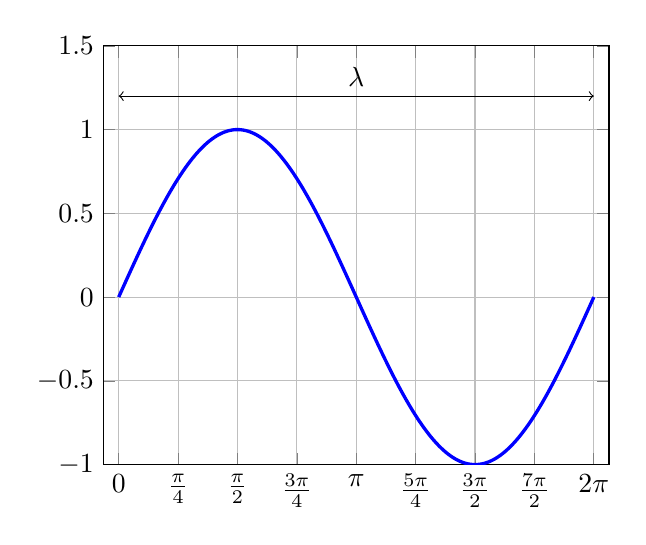
\begin{tikzpicture}
	\begin{axis}
		[
		xmin=-0.2,
		xmax=2*pi+0.2,
		ymin=-1,
		ymax=1.5,
		no marks,grid,
		xticklabels={0, $\frac{\pi}{4}$,  $\frac{\pi}{2}$,
			$\frac{3\pi}{4}$, $\pi$,$\frac{5\pi}{4}$,
			$\frac{3\pi}{2}$, $\frac{7\pi}{2}$, 2$\pi$},
		xtick={0, 0.7853,...,6.2832},
		]
		\addplot[blue,very thick,samples=200,domain=0:2*pi]{sin(deg(x))};
		\draw[<->]      (0,1.2) -- node[above] {$\lambda$} (6.2832,1.2);
	\end{axis}
\end{tikzpicture}
